\tikzset{fontscale/.style = {font=\relsize{#1}}
    }
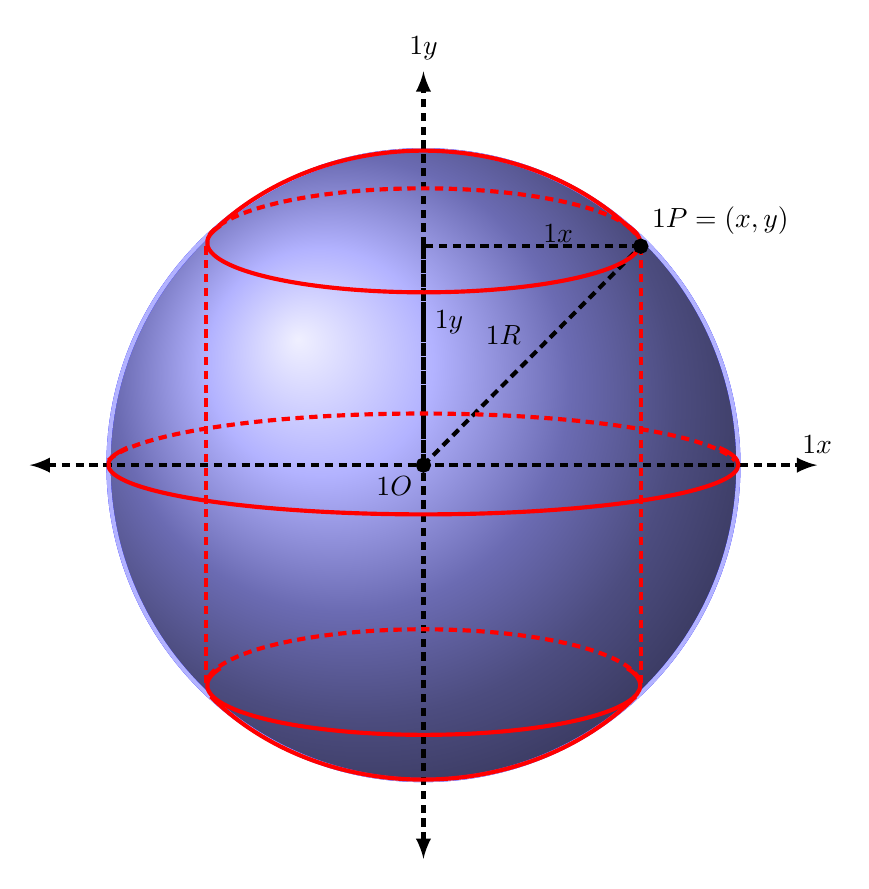
\begin{tikzpicture}[font = \sansmath,fontscale=1,scale=2,line width=1.5pt]
%\draw [very thin, style=gray!50, step=0.5] (-3,-2) grid (3,2);
  \coordinate (O) at (0,0);
 \coordinate (A) at (-1.38,1.39);
 \coordinate (B) at (-1.38,-1.39);
 \coordinate (C) at (1.38,1.39);
 \coordinate (D) at (1.38,-1.39);
\coordinate (E) at (0,1.39);

%%%axis
  % ball background color
 \shadedraw[shading=ball,ball color=blue!40, blue](0,0) circle [radius = 2cm];
  

  % ball
  \draw [blue!30](O) circle [radius=2cm];
  
  % radius
  \draw[densely dashed] (O) to [edge label = $R$] (C);
 % \draw[densely dashed,gray!30] (O) -- (1.33,1.33);
% label of ball center point
  \filldraw (O) circle (1pt) node[below left] {$O$};
 
%cilindro
 \draw[densely dashed,red] (A) to (B);
\draw[densely dashed,red] (C) to  (D);
\draw[densely dashed] (C) to [above=12pt,edge label = $x$] (E);
\draw[densely dashed] (E) to [above=12pt,edge label = $y$] (O);
%%%%%axis
\draw[densely dashed,latex-latex] (0,-2.5) -- (0,2.5)node[above]{$y$};
\draw[densely dashed,latex-latex] (-2.5,0) -- (2.5,0)node[above]{$x$};
  % cut of ball surface top
  \draw[red] (-1.35,1.47) arc [start angle = 140, end angle = 40,
    x radius = 17.6mm, y radius = 14.75mm];
  \draw[red, densely dashed] (-1.36,1.46) arc [start angle = 170, end angle = 10,
    x radius = 13.8mm, y radius = 3.6mm];
  \draw[red] (-1.29,1.52) arc [start angle=-200, end angle = 20,
    x radius = 13.75mm, y radius = 3.15mm];
% cut of ball surface botton
  \draw[red] (-1.35,-1.47) arc [start angle = -140, end angle = -40,
    x radius = 17.6mm, y radius = 14.75mm];
  \draw[red, densely dashed] (-1.36,-1.34) arc [start angle = 170, end angle = 10,
    x radius = 13.8mm, y radius = 3.6mm];
  \draw[red] (-1.29,-1.29) arc [start angle=-200, end angle = 20,
    x radius = 13.75mm, y radius = 3.15mm];

%centro of ball 
 \draw[red, densely dashed] (-2,0.03) arc [start angle = 170, end angle = 10,
    x radius = 20.2mm, y radius = 3.6mm];
  \draw[red] (-1.88,0.11) arc [start angle=-200, end angle = 20,
    x radius = 20mm, y radius = 3.15mm];
%%%%%%%%%%%% Punto
 \filldraw (C) circle (1pt) node[above right] {$P=(x,y)$};
\end{tikzpicture}
